\documentclass[../../main/main.tex]{subfiles}
\graphicspath{{./figures/}}

\dominitoc
\faketableofcontents

\makeatletter
\renewcommand{\@chapapp}{Optique -- chapitre}
\makeatother

\toggletrue{student}
\HideSolutionstrue

\begin{document}
\setcounter{chapter}{2}

\chapter{Miroir plan et lentilles minces}

\vfill

\begin{prgm}
	\begin{tcb}*(ror)"know"{Savoirs}
		\begin{itemize}[label=$\diamond$, leftmargin=10pt]
			\item Connaître les propriétés d'un miroir plan.
			\item Définir les propriétés du centre optique, des foyers principaux et
			      secondaires, de la distance focale, de la vergence.
			\item Prévoir par construction graphique et par application successive de
			      relations de conjugaison et/ou de grandissement la position et la taille
			      d’une image par un système optique composé de plusieurs lentilles.
		\end{itemize}
	\end{tcb}

	\begin{tcb}*(ror)"how"{Savoir-faire}
		\begin{itemize}[label=$\diamond$, leftmargin=10pt]
			\item Construire l’image d’un objet par un miroir plan.
			\item Construire l’image d’un objet situé à distance finie ou infinie à
			      l’aide de rayons lumineux, identifier sa nature réelle ou virtuelle.
			\item Exploiter les formules de conjugaison et de grandissement
			      transversal de Descartes et de Newton.
			\item Établir et utiliser la condition de formation de l’image réelle
			      d’un objet réel par une lentille convergente.
		\end{itemize}
	\end{tcb}
\end{prgm}

\vfill
\minitoc
\vfill

\newpage

\section{Miroir plan}
\subsection{Définition}

\begin{tcbraster}[raster columns=2, raster equal height=rows]
	\begin{tcb}[label=def:mir](defi){Miroir plan}
		Surface plane totalement réfléchissante. On le schématisme avec le symbole
		\begin{center}
			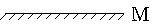
\includegraphics[width=4cm]{mir_plan}
		\end{center}
		pour un miroir orienté vers le haut.
	\end{tcb}
	\begin{tcb}[label=mirstig](ror)'r'{Stigmatisme, aplanétisme}
		Le miroir plan est le seul système optique \textbf{rigoureusement} stigmatique et
		aplanétique.
	\end{tcb}
\end{tcbraster}

\subsection{Construction d'images}
On utilise les lois de Snell-Descartes pour la réflexion, en traçant deux rayons
partant de l'objet ponctuel.

\begin{tcb}[label=prop, sidebyside, righthand ratio=.4](prop){Image d'un objet réel}
	Soit \textbf{A un point objet} d'un miroir plan. Les rayons \textbf{incidents}
	se croisant en A arrivent sur le miroir en I et I'. Par la loi de la
	\textbf{réflexion}, les rayons émergents sont les rayons réfléchis, avec un
	angle de réflexion \textbf{opposé} à l'angle d'incidence. On trouve
	\textbf{l'image A'} en traçant l'intersection des rayons \textbf{émergents}.
	\bigbreak
	Avec la figure ci-contre, on observe
	\psw{
		\[
			\tan(i) =
			\frac{\obar{\rm HI}}{\obar{\rm HA}} =
			\frac{\obar{\rm HI}}{-\obar{\rm HA'}}
		\]
	}
	Soit
	\psw{
		\[
			\boxed{\obar{\rm HA'} = -\obar{\rm HA}}
		\]
	}
	\tcblower
	\begin{center}
		\switch{
			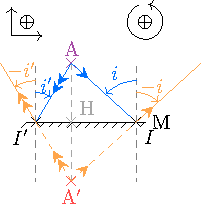
\includegraphics[width=.8\linewidth, draft=true]{mir_plan-obj_r}
		}{
			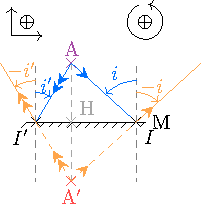
\includegraphics[width=.8\linewidth]{mir_plan-obj_r}
		}
		\captionof{figure}{Image d'un objet R.\ par un miroir plan.}
		\label{fig:mir_plan-obj_r}
	\end{center}
\end{tcb}

\begin{tcb}[label=prop, sidebyside, righthand ratio=.4](prop){Image d'un objet
			virtuel}
	Le principe du retour inverse de la lumière permet de permuter A et A'
	dans la démonstration précédente.
	\tcblower
	\begin{center}
		\switch{
			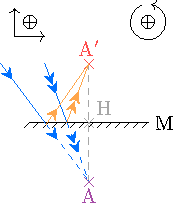
\includegraphics[width=.8\linewidth, draft=true]{mir_plan-obj_v}
		}{
			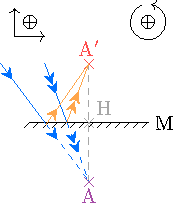
\includegraphics[width=.8\linewidth]{mir_plan-obj_v}
		}
		\captionof{figure}{Image d'un objet V.\ par un miroir plan.}
		\label{fig:mir_plan-obj_v}
	\end{center}
\end{tcb}

\subsection{Relation de conjugaison}


\begin{tcb}[label=def:relconj](defi){Relation de conjugaison}
	Formule mathématique reliant la position d'un objet à celle de son image
	par un système optique.
\end{tcb}
\begin{tcb}*[label=prop:mirconj](prop)"ror"{Relation de conjugaison d'un miroir plan}
	L'image A' par un miroir plan est le \textbf{symétrique} de l'objet
	A. Avec H le projeté orthogonal de A sur le miroir plan, on écrit
	cette conjugaison
	\[
		\psw{
			\boxed{\rm A \opto{\rm M}{\rm H} A'}
		}
		\qav
		\psw{
			\boxed{\obar{\rm HA'} = -\obar{\rm HA}}
		}
	\]
\end{tcb}
\begin{tcb}[label=rema:mirrv](rema){Réalité et virtualité du miroir plan}
	Le miroir plan \textbf{garde la nature d'un faisceau}~: s'il est divergent en
	entrée, il est divergent en sortie et inversement. Ainsi, avec la définition
	du caractère réel et virtuel des objets, \textbf{le miroir plan change la
		nature de l'objet}.
\end{tcb}

\subsection{Grandissement transversal}

\begin{tcb}[label=prop:mir_grand](prop){$\gamma$ miroir plan}
	Le miroir plan a un grandissement transversal
	\psw{
		\[
			\boxed{\gamma = +1}
		\]
	}
	\vspace{-20pt}
\end{tcb}
\begin{tcb}[label=demo:mir_grand, sidebyside,
		righthand ratio=.4](demo){$\gamma$ miroir plan}
	Soit AB un objet étendu. On construit son image A'B' par le miroir plan~: on
	appelle H le projeté orthogonal de A sur le miroir, H' celui de B.
	\smallbreak
	On a
	\[
		\psw{
			\obar{\rm BH'} = \obar{\rm H'B}
		}
		\qet
		\psw{
			\obar{\rm AH} = \obar{\rm HA'}
		}
	\]
	Ainsi, on obtient
	\psw{
		\[
			\boxed{\AB = \obar{\rm HH'} = \ABp}
		\]
	}
	\tcblower
	\begin{center}
		\switch{
			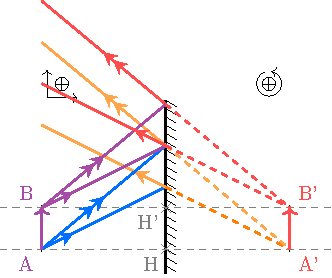
\includegraphics[width=\linewidth, draft=true]{mir_plan-grand}
		}{
			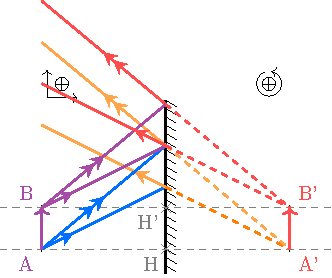
\includegraphics[width=\linewidth]{mir_plan-grand}
		}
		\captionof{figure}{Image d'un objet étendu par un miroir plan.}
		\label{fig:mir_plan-grand}
	\end{center}
\end{tcb}

\section{Lentilles minces}
\subsection{Définition}

\begin{tcb}[label=def:lents](defi){Lentilles, minces, convergentes et divergentes}
	Une lentille est un composant optique \textbf{centré} constitué d'un milieu
	TLHI, délimité par deux dioptres de sommets S$_1$ et S$_2$. Elle est dite
	\textbf{mince} si son diamètre est très grand devant son épaisseur.
	\smallbreak
  \begin{isd}[sidebyside align=top]
		\tcbsubtitle{\fatbox{Convergente}}
		Son \textbf{point foyer objet} est \textbf{avant sa face d'entrée}.
		\begin{center}
			\switch{
				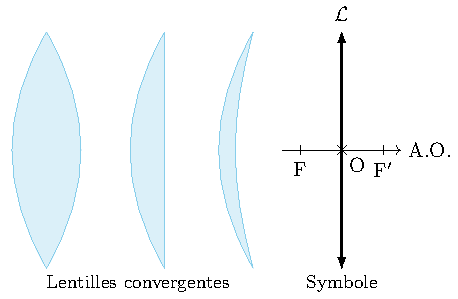
\includegraphics[height=4cm, draft=true]{lent_conv-def}
			}{
				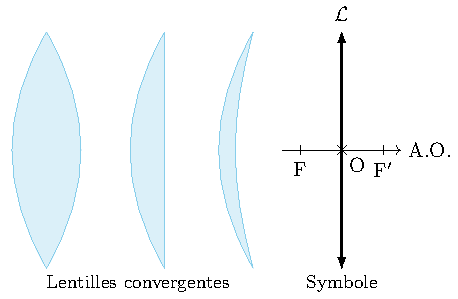
\includegraphics[height=4cm]{lent_conv-def}
			}
			\captionof{figure}{Exemples de lentilles convergentes.}
			\label{fig:lent_conv-def}
		\end{center}
		\tcblower
		\tcbsubtitle{\fatbox{Divergente}}
		Son \textbf{point foyer objet} est \textbf{après sa face de sortie}.
		\begin{center}
			\switch{
				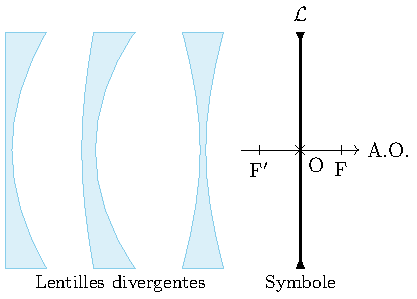
\includegraphics[height=4cm, draft=true]{lent_div-def}
			}{
				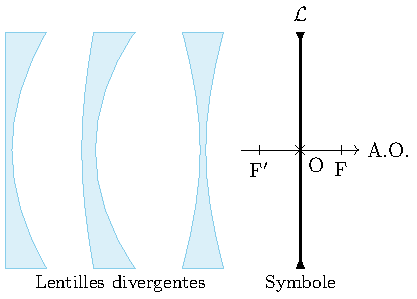
\includegraphics[height=4cm]{lent_div-def}
			}
			\captionof{figure}{Exemples de lentilles divergentes.}
			\label{fig:lent_conv-def}
		\end{center}
	\end{isd}
\end{tcb}


\begin{tcb}[label=rema:lent_gauss](rema){Stigmatisme et aplanétisme}
	D'une manière générale, les lentilles minces ne sont ni stigmatiques ni
	aplanétiques. Nous utiliserons donc toujours les lentilles minces dans
	les \textbf{conditions de Gauss} et les considérerons comme stigmatiques
	et aplanétiques.
\end{tcb}

\subsection{Caractéristiques}

\begin{tcbraster}[raster columns=2, raster equal height=rows]
	\begin{tcb}[label=def:co](defi){Centre optique}
		\psw{
			On appelle \textbf{centre optique} d'une lentille et on le note $O$ le
			point à l'intersection de l'axe optique et de la lentille.
		}
	\end{tcb}
	\begin{tcb}[label=prop:co](prop)'r'{Centre optique et foyers}
		\psw{
			Tout rayon passant par le centre optique $O$ d'une lentille mince
			\textbf{n'est pas dévié}, et $F'$ est \textbf{symétrique} de $F$ par
			$O$.
		}
	\end{tcb}
	\begin{tcb}[label=def:fv, raster multicolumn=2](defi){Distance focale image
				et vergence}
		\begin{isd}
			On appelle \textit{distance focale image} la distance
			\textbf{algébrique} $\OFp$~; elle est positive pour une lentille
			convergent, négative pour une lentille divergente. \textbf{Elle se
				note usuellement $f'$}.
			\tcblower
			On appelle \textit{vergence} et on note $V$ la grandeur définie par
			\psw{
				\[
					\boxed{V = \frac{1}{\OFp}}
				\]
			}
		\end{isd}
		\tcbsubtitle{\fatbox{Unités}}
		\begin{isd}
			\psw{
				En tant que distance, $\OFp$ (ou $f'$) s'exprime en mètres (m).
			}
			\tcblower
			\psw{
				L'unité de la vergence est le \si{m^{-1}}, mais elle s'exprime
				usuellement en \textbf{dioptries} ($\delta$).
			}
		\end{isd}
	\end{tcb}
\end{tcbraster}

\subsection{Constructions géométriques d'une lentille mince}
\subsubsection{Rappel}

\begin{tcb}[label=rapp:foy](rapp){Foyers d'une lentille}

	Par définition (voir chapitre 2), le \textbf{foyer objet} $F$ donne une
	\textbf{image à l'infini}, et ce \textbf{\underline{peu importe la nature de
			la lentille}}.\bigbreak

	De même, le \textbf{foyer image} $F'$ est le point \textbf{image} d'un
	\textbf{objet à l'infini}.

\end{tcb}
\begin{tcb}[label=exem:lentfoy, sidebyside](exem){Foyers des lentilles}
	\begin{center}
		\switch{
			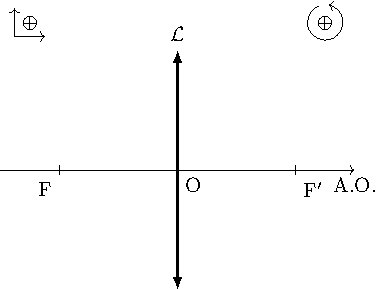
\includegraphics[width=\linewidth]{lent_conv-Fp_plain}
		}{
			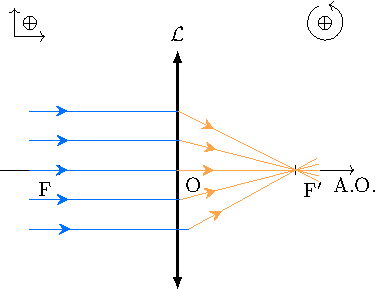
\includegraphics[width=\linewidth]{lent_conv-Fp}
		}
		\captionof{figure}{Foyer image convergent}
		\label{fig:convfp}
	\end{center}
	\tcblower
	\begin{center}
		\switch{
			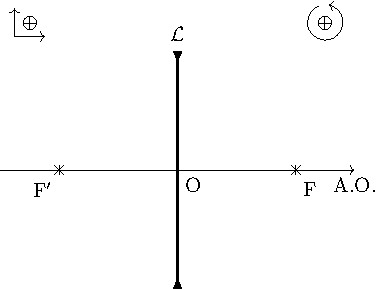
\includegraphics[width=\linewidth]{lent_div-Fp_plain}
		}{
			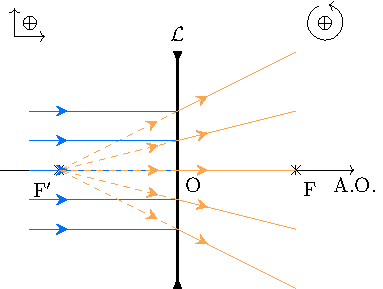
\includegraphics[width=\linewidth]{lent_div-Fp}
		}
		\captionof{figure}{Foyer image divergent}
		\label{fig:divfp}
	\end{center}
\end{tcb}

\subsubsection{Règles primaires}

\begin{tcbraster}[raster columns=2, raster equal height=rows]
	\begin{tcb}[label=impo:lent_regles](ror){Règles primaires}
		Avec la propriété des foyers principaux, on a donc 3 points d'intérêts
		pour construire les rayons émergents d'une lentille mince~:
		\begin{enumerate}
			\item \psw{Tout rayon incident passant par $O$ n'est pas dévié~;}
			\item \psw{Tout rayon incident parallèle à l'axe optique émerge en
				      passant par $F'$.}
			\item \psw{Tout rayon incident passant par $F$ émerge parallèle à l'axe
				      optique~;}
		\end{enumerate}
	\end{tcb}
	\begin{tcb}[label=exem:constru](exem)'r'{Cas simple}
		\begin{center}
			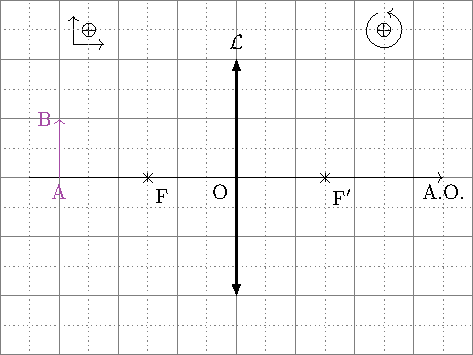
\includegraphics[width=\linewidth]{lent_conv-constru_simple-plain}
			\captionof{figure}{Utilisation des règles primaires}
			\label{fig:convconstrusimple}
		\end{center}
	\end{tcb}
\end{tcbraster}
\begin{tcb}[label=impo:cons_exem](impo){Exemples de situations à compléter}
	\begin{minipage}{0.50\linewidth}
		\begin{center}
			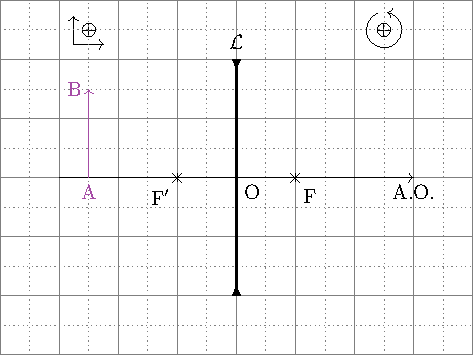
\includegraphics[width=\linewidth]{lent_div-constru_simple-plain}
			\captionof{figure}{Divergente simple}
			\label{fig:divconstrusimple}
		\end{center}
	\end{minipage}
	\hfill
	\begin{minipage}{0.50\linewidth}
		\begin{center}
			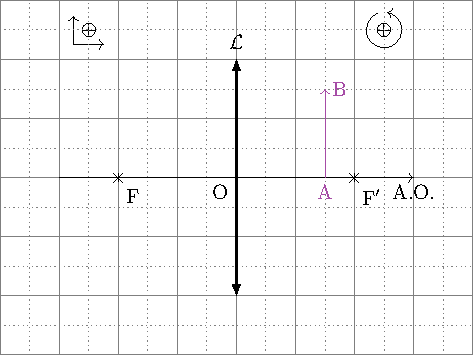
\includegraphics[width=\linewidth]{lent_conv-constru_after-plain}
			\captionof{figure}{Convergente après}
			\label{fig:convconstruafter}
		\end{center}
	\end{minipage}
	\begin{minipage}{0.50\linewidth}
		\begin{center}
			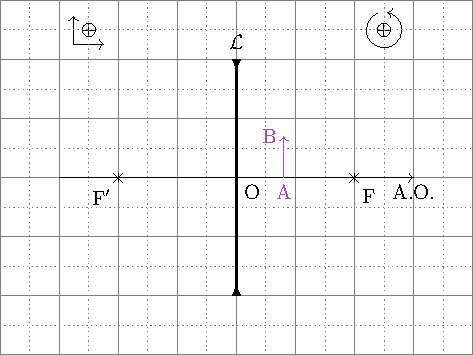
\includegraphics[width=\linewidth]{lent_div-constru_after_a-plain}
			\captionof{figure}{Divergente après}
			\label{fig:divconstruafter}
		\end{center}
	\end{minipage}
	\hfill
	\begin{minipage}{0.50\linewidth}
		\begin{center}
			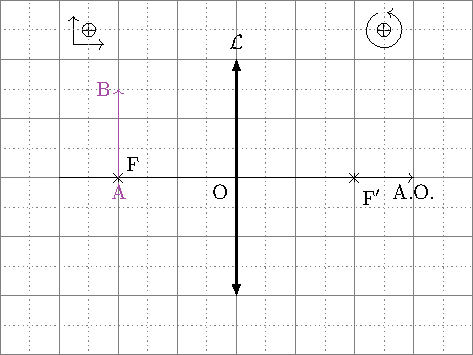
\includegraphics[width=\linewidth]{lent_conv-constru_F-plain}
			\captionof{figure}{Convergente $F$}
			\label{fig:convconstruF}
		\end{center}
	\end{minipage}
\end{tcb}

\subsubsection{Règles secondaires}
\begin{tcbraster}[raster columns=2, raster equal height=rows]
	\begin{tcb}[label=impo:lent_regles, hand](ror){Règles secondaires}
		Avec la propriété des foyers secondaires, on a deux règles de
		construction supplémentaires~:
		\begin{enumerate}[start=4]
			\item \psw{Deux rayons incidents parallèles entre eux émergent en se
				      croisant dans le plan focal image~;}
			\item \psw{Deux rayons incidents se croisant dans le plan focal objet
				      émergent parallèles entre eux.}
		\end{enumerate}
	\end{tcb}
	\begin{tcb}[label=exem:constru](exem)'r'{Cas simple}
		\begin{center}
			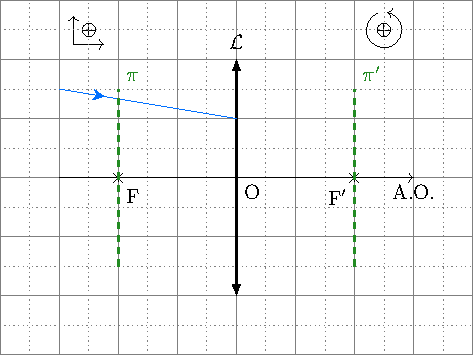
\includegraphics[width=\linewidth]{lent_conv-qqe-plain}
			\captionof{figure}{Utilisation des règles secondaires}
			\label{fig:convconstruqqe}
		\end{center}
	\end{tcb}
\end{tcbraster}

\subsubsection{Corrigé des tracés}

\begin{tcb}[label=exem, sidebyside](exem){Cas simple}
	\begin{center}
		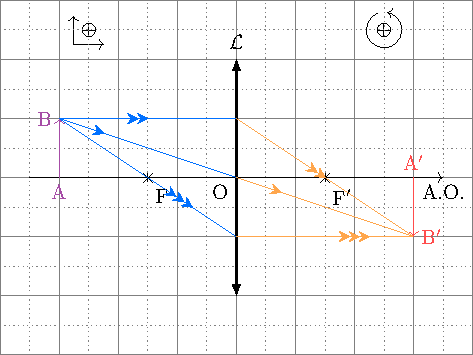
\includegraphics[width=\linewidth]{lent_conv-constru_simple}
		\captionof{figure}{Utilisation des règles primaires}
		\label{fig:corrconvconstrusimple}
	\end{center}
	\tcblower
	\begin{center}
		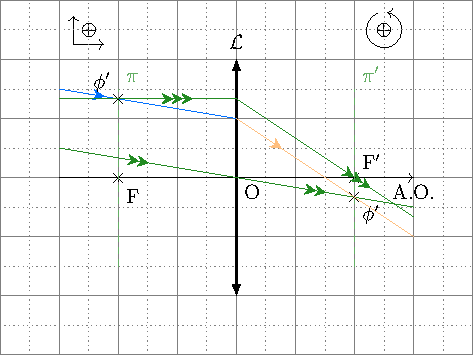
\includegraphics[width=\linewidth]{lent_conv-qqe}
		\captionof{figure}{Utilisation des règles secondaires}
		\label{fig:convconstruqqe}
	\end{center}
\end{tcb}
\begin{tcb}[label=impo:cons_exem](impo){Exemples de situations à compléter}
	\begin{minipage}{0.50\linewidth}
		\begin{center}
			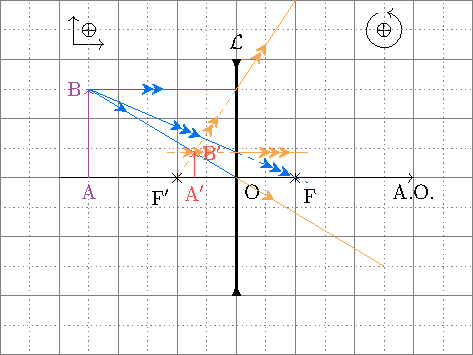
\includegraphics[width=\linewidth]{lent_div-constru_simple}
			\captionof{figure}{Divergente simple}
			\label{fig:corrdivconstrusimple}
		\end{center}
	\end{minipage}
	\hfill
	\begin{minipage}{0.50\linewidth}
		\begin{center}
			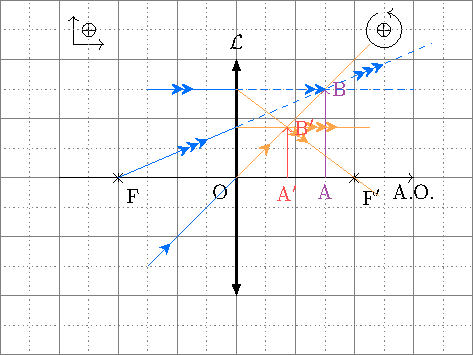
\includegraphics[width=\linewidth]{lent_conv-constru_after}
			\captionof{figure}{Convergente après}
			\label{fig:corrconvconstruafter}
		\end{center}
	\end{minipage}
	\begin{minipage}{0.50\linewidth}
		\begin{center}
			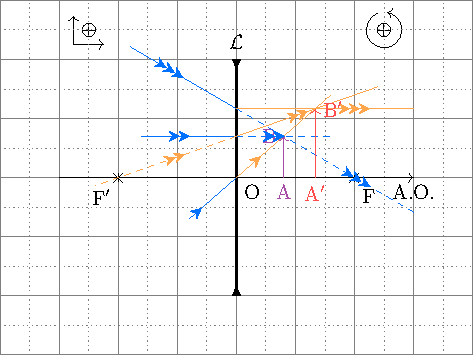
\includegraphics[width=\linewidth]{lent_div-constru_after_a}
			\captionof{figure}{Divergente après}
			\label{fig:corrdivconstruafter}
		\end{center}
	\end{minipage}
	\hfill
	\begin{minipage}{0.50\linewidth}
		\begin{center}
			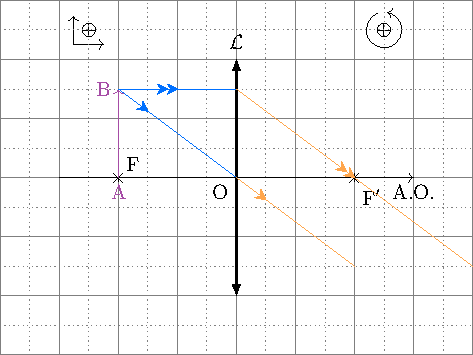
\includegraphics[width=\linewidth]{lent_conv-constru_F}
			\captionof{figure}{Convergente $F$}
			\label{fig:corrconvconstruF}
		\end{center}
	\end{minipage}
\end{tcb}

\subsection{Relations de conjugaisons}

\begin{tcb}*[label=prop:conjdescartes](prop)"ror"{Relations de conjugaison}
	Soit $\mathcal{L}$ une lentille de centre optique O et de foyers F
	et F', réalisant l'image A' d'un objet A. On écrit
	\psw{
		\[
			\boxed{\rm A \opto{\Lc}{\rm O} A'}
		\]
	}
	et on a
	\smallbreak
	\begin{isd}
		\tcbsubtitle{\fatbox{Relation de \textsc{Descartes}, au centre}}
		\psw{
			\[
				\boxed{ \frac{1}{\OFp} = \frac{1}{\OAp} - \frac{1}{\OA}}
			\]
		}
		% Relation de conjugaison de Descartes, avec origine au centre.
		\tcblower
		\tcbsubtitle{\fatbox{Relation de \textsc{Newton}, au foyer}}
		\psw{
			\begin{empheq}[box=\fbox]{align*}
				\OFp\times\OF    & = \obar{\rm F'A'}\obar{\rm FA}\\
				\Leftrightarrow -f'^2 & = \obar{\rm F'A'}\obar{\rm FA}
			\end{empheq}
		}
		% Relation de conjugaison de Newton, avec origine aux foyers
	\end{isd}
\end{tcb}

\subsection{Grandissement transversal}

\begin{tcb}[label=coro:lent_grand](prop){$\gamma$ lentille mince}
	À partir de la définition du grandissement transversal $\gamma =
		\frac{\ABp}{\AB}$, on peut définir

	\begin{isd}
		\psw{
			\[
				\boxed{\gamma = \frac{\ABp}{\AB} = \frac{\OAp}{\OA}}
			\]
		}
		\tcblower
		\psw{
			\[
				\boxed{
					\gamma =
					\frac{\obar{\rm F'A'}}{\obar{\rm F'O}} =
					\frac{\obar{\rm FO}}{\obar{\rm FA}}}
			\]
		}
	\end{isd}
\end{tcb}

\subsection{Complément~: démonstrations des relations}

\begin{tcb}[label=demo:lent_rc, breakable](demo){Relations de conjugaison et grandissement}
	\begin{isd}
		Soit $\Lc$ telle que $\rm AB \opto{\Lc}{\rm O} A'B'$. On a la figure
		ci-contre.

		Pour trouver la relation de conjugaison, nous utilisons les triangles
		OAB et OA'B' pour lesquels nous utilisons le théorème de \textsc{Thalès}.
		Nous avons directement la formule du grandissement de Descartes~:
		\psw{
			\[
				\boxed{
					\frac{\ABp}{\AB} =
					\frac{\OAp}{\OA} = \gamma
				}
			\]
		}
		\tcblower
		\begin{center}
			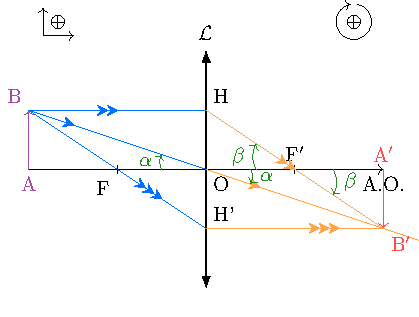
\includegraphics[width=\linewidth]{lent_conv-demo}
			\captionof{figure}{Schéma de notations}
			\label{fig:lent_rc}
		\end{center}
	\end{isd}
	Nous définissons ensuite le point H projeté orthogonal de B sur
	la lentille, et le point H' projeté orthogonal de B' sur la lentille.
	\smallbreak
	\begin{isd}
		En utilisant le théorème de \textsc{Thalès} dans les triangles F'OH et
		F'A'B' et en remarquant que $\obar{\rm OH} = \AB$, on a cette fois
		\psw{
			\begin{gather*}
				\frac{\obar{\rm A'B'}}{\obar{\rm OH}} = \frac{\ABp}{\AB} =
				\frac{\obar{\rm F'A'}}{\obar{\rm F'O}}
				\\\Lra
				\boxed{\gamma = - \frac{\obar{\rm F'A'}}{\OFp}}
			\end{gather*}
		}
		\tcblower
		Et en utilisant les triangles FAB et FOH'
		\psw{
			\begin{gather*}
				\frac{\obar{\rm OH'}}{\obar{\rm AB}} = \frac{\ABp}{\AB} =
				\frac{\obar{\rm FO}}{\obar{\rm FA}}
				\\\Lra
				\boxed{\gamma = - \frac{\OF}{\obar{\rm FA}}}
			\end{gather*}
		}
	\end{isd}
	En les combinant on obtient élémentairement
	\psw{
		\begin{empheq}[box=\fbox]{align*}
			\OFp\times\OF    & = \obar{\rm F'A'}\obar{\rm FA}\\
			\Leftrightarrow -f'^2 & = \obar{\rm F'A'}\obar{\rm FA}
		\end{empheq}
	}
	En y injectant les décompositions
	\begin{equation*}
		\obar{\rm F'A'} = \psw{
			\obar{\rm F'O} + \obar{\rm OA'}
		}
		\qet
		\obar{\rm FA} = \psw{
			\obar{\rm FO} + \obar{\rm OA}
		}
	\end{equation*}
	et après développement, on obtient
	\begin{equation*}
		\OFp\OAp - \OFp\OA + \OA\OAp = 0
		\iff
		\psw{
			\boxed{
				\frac{1}{\OFp} = \frac{1}{\OAp} - \frac{1}{\OA}
			}
		}
	\end{equation*}
	par division par $\OFp\OA\OAp$.
\end{tcb}

\section{Quelques applications}

\subsection{Condition de netteté}

Soit $\ABr \opto{\Lc}{\rm O} \ABpr$ avec $\Lc$ convergente projetant sur un écran. On
appelle $x$ la distance $ \abs{\OA}$ et $D$ la distance fixe AA'.
Quelle est la contrainte sur le choix de lentille pour que A'B' soit nette~?

\begin{tcbraster}[raster columns=2, raster equal height=rows]
	\begin{tcb}[](data){Données}
		\begin{center}
			\switch{
				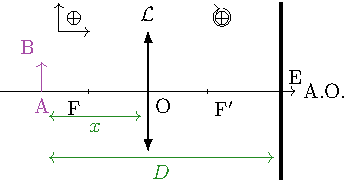
\includegraphics[width=\linewidth]{lent_conv-condition_plain}
			}{
				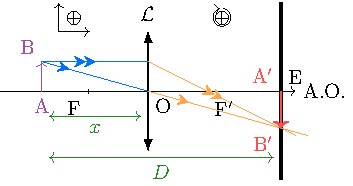
\includegraphics[width=\linewidth]{lent_conv-condition}
			}
			\captionof{figure}{Schéma de situation}
			\label{fig:lent_condi}
		\end{center}
	\end{tcb}
	\begin{tcolorbox}[blankest, raster multicolumn=1, space to=\myspace]
		\begin{tcbraster}[raster columns=1]
			\begin{tcb}[add to natural height=\myspace](ques)'r'{Résultat attendu}
				\psw{
					L'image est nette si la lentille forme l'image sur l'écran. Avec
					$D$ fixe, on cherche une équation avec $x$.
				}
			\end{tcb}
			\begin{tcb}[add to natural height=\myspace](tool)'r'{Outils}
				\psw{
					Relation de Descartes
					\[
						\boxed{ \frac{1}{\OFp} = \frac{1}{\OAp} - \frac{1}{\OA}}
					\]
					et $\OA = -x$, $\OAp = D-x$.
				}
			\end{tcb}
		\end{tcbraster}
	\end{tcolorbox}
\end{tcbraster}

\begin{tcb}[sidebyside](appl){Application}
	Avec les notations de l'énoncé, la relation de Descartes devient
	\psw{
		\begin{align*}
			\frac{1}{f'}                 & = \frac{1}{D-x} - \frac{1}{-x} \\
			\Leftrightarrow \frac{1}{f'} & = \frac{x + D-x}{x(D-x)}       \\
			\Leftrightarrow f'           & = \frac{x(D-x)}{D}             \\
			\Leftrightarrow 0            & = x^2 - xD + f'D
		\end{align*}
	}
	Ce trinôme du second degré a pour discriminant
	\psw{
		\[
			\boxed{\Delta = D^2-4f'D = D(D-4f')}
		\]
	}
	\tcblower
	$x$ étant une distance physique, on cherche $\Delta \geq 0$.
	\begin{itemize}[label=$\diamond$, leftmargin=10pt]
		\item $\Delta = 0$ si $D = 4f'$, et alors
		      \psw{
			      \[
				      \boxed{x = \frac{D}{2}}
			      \]
		      }
		      \vspace{-20pt}
		\item $\Delta > 0$ si $D > 4f'$, et alors
		      \psw{
			      \[
				      \boxed{x_\pm = \frac{D\pm\sqrt{D(D-4f')}}{2}}
			      \]
		      }
		      \vspace{-20pt}
	\end{itemize}
	Ainsi, la zone de netteté de l'image se situe entre $x_+$ et $x_-$, et a
	donc une largeur
	\psw{
		\[
			\boxed{d = x_+ - x_- = \sqrt{D(D-4f')}}
		\]
	}
	\vspace{-20pt}
\end{tcb}

\subsection{Champ de vision à travers un miroir plan}
Une personne dont les yeux se situent à $h = \SI{1.70}{m}$ du sol observe une
mare gelée (équivalente à un miroir plan) de largeur $l = \SI{5.00}{m}$ et
située à $d = \SI{2.00}{m}$ d'elle.
\begin{enumerate}
	\item Peut-elle voir sa propre image~? Quelle est la nature de l'image~?
	\item Quelle est la hauteur maximale $H$ d'un arbre situé de l'autre côté de
	      la mare (en bordure de mare) qu'elle peut voir par réflexion dans la
	      mare~? On notera $D = l+d$.
\end{enumerate}

\subsubsection{Propre image}
\begin{tcbraster}[raster columns=2, raster equal height=rows]
	\begin{tcb}(data){Schéma}
		\begin{center}
			\switch{
				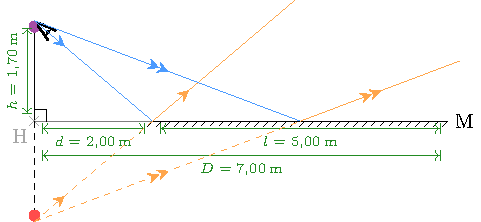
\includegraphics[width=\linewidth, draft=true]{ch3-arbre-1}
			}{
				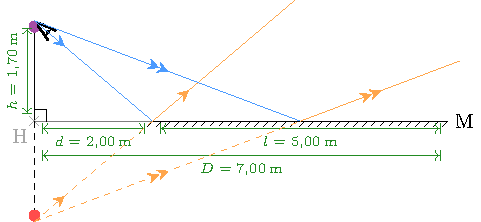
\includegraphics[width=\linewidth]{ch3-arbre-1}
			}
		\end{center}
	\end{tcb}
	\begin{tcolorbox}[blankest, raster multicolumn=1, space to=\myspace]
		\begin{tcbraster}[raster columns=1]
			\begin{tcb}(tool)'r'{Outil}
				Pour voir une image, il faut qu'un rayon partant de l'image
				puisse arriver jusqu'à l'œil de l'observataire. Étant donné
				qu'on travaille avec un miroir, l'image de l'observataire est
				son symétrique par le plan du miroir (même si le miroir ne
				s'étend pas jusque-là !).
			\end{tcb}
			\begin{tcb}(appl)'r'{Application}
				\psw{
					On voit vite qu'il n'est pas possible qu'un rayon issu de
					l'image (en rouge) atteigne l'œil (en violet). On comprend par
					le tracé des rayons réfléchis que seul l'autre côté du lac sera
					visible.
				}
			\end{tcb}
		\end{tcbraster}
	\end{tcolorbox}
\end{tcbraster}

\subsubsection{Image arbre}
\begin{tcbraster}[raster columns=2, raster equal height=rows]
	\begin{tcb}(data){Schéma}
		\begin{center}
			\switch{
				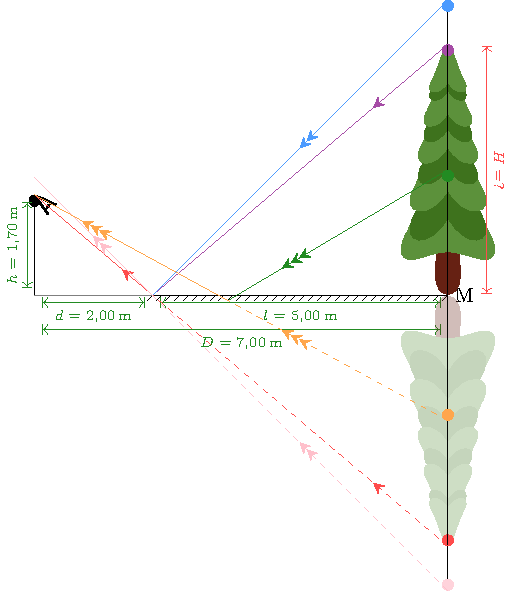
\includegraphics[width=\linewidth, draft=true]{ch3-arbre-2}
			}{
				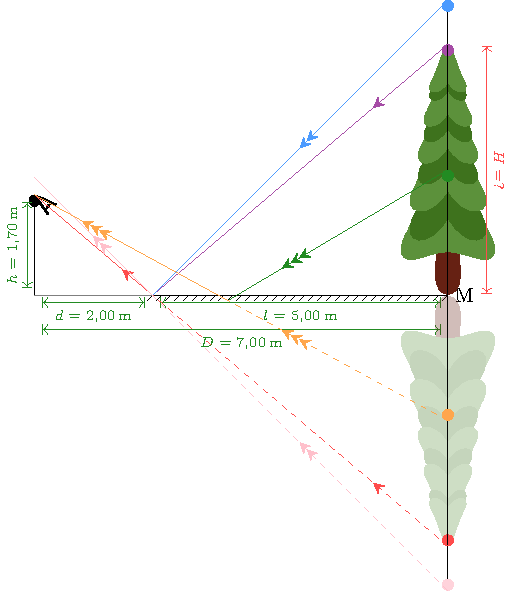
\includegraphics[width=\linewidth]{ch3-arbre-2}
			}
		\end{center}
	\end{tcb}
	\begin{tcolorbox}[blankest, raster multicolumn=1, space to=\myspace]
		\begin{tcbraster}[raster columns=1]
			\begin{tcb}[add to natural height=\myspace](tool)'r'{Outil}
				Ici aussi, l'idée est de trouver l'image de l'arbre, et de voir
				la condition limite pour la taille visible.
			\end{tcb}
			\begin{tcb}(appl)'r'{Application}
				\psw{
					Un schéma avec l'image de l'arbre nous permet de voir que le
					point le plus haut qu'on peut voir par réflexion sur le lac est
					quand on regarde proche de nous : si on regarde plus loin, on
					voit en effet plus vers le bas de l'arbre (rayon vert incident,
					rayon orange émergent). Un arbre qui est trop grand ne sera pas
					visible en regardant ce point-là (rayon bleu incident, rose
					émergent). On s'intéresse donc à la construction géométrique
					formée par le rayon violet incident, rouge émergent, qui nous
					permet d'appliquer le théorème de Thalès : $\DS\frac{H}{l} =
						\frac{h}{d}$, soit
					\[
						\boxed{H = \frac{l\times h}{d}}
						\qav
						\left\{
						\begin{array}{rcl}
							l & = & \SI{5.00}{m} \\
							h & = & \SI{1.70}{m} \\
							d & = & \SI{2.00}{m}
						\end{array}
						\right.
					\]
					D'où
					\[
						\xul{H = \SI{4.25}{m}}
					\]
				}
        \vspace{-20pt}
			\end{tcb}
		\end{tcbraster}
	\end{tcolorbox}
\end{tcbraster}

\end{document}
